% MMA3001 project report -- initial draft.
% Red [TODO: ...] notes mark things only you can fill in or must check before submission.
\documentclass[11pt, a4paper]{article}
\renewcommand{\abstractname}{Summary}
\usepackage{graphicx,caption,parskip}
\usepackage[nodayofweek,level]{datetime}
\usepackage{placeins}
\usepackage[toc,page]{appendix}
\usepackage{amsmath,booktabs,xcolor,enumitem,array}
\newcolumntype{L}[1]{>{\raggedright\arraybackslash}p{#1}}
\setlist{nosep}
\setlength{\textfloatsep}{10pt plus 2pt minus 2pt}
\renewcommand{\topfraction}{0.85}      % floats may fill up to 85% of a page top
\renewcommand{\bottomfraction}{0.7}    % ...or 70% at the bottom
\renewcommand{\textfraction}{0.1}      % a page needs only 10% text
\renewcommand{\floatpagefraction}{0.85}% float-only pages must be 85% full
\setcounter{page}{0}
\usepackage[backend=biber, style=phys, giveninits=true, isbn=false,url=false,doi=false, biblabel=brackets]{biblatex}
\usepackage[colorlinks]{hyperref}
\hypersetup{
    urlcolor = cyan,
    citecolor = blue,
    linkcolor = blue
}
\usepackage{geometry}
\newgeometry{vmargin={20mm}, hmargin={22mm,22mm}}

\addbibresource{references.bib}
\graphicspath{{reports/figures/}}

\newcommand{\todo}[1]{\textcolor{red}{[TODO: #1]}}
\newcommand{\mydate}{\formatdate{25}{10}{2026}}

\title{\textbf{A Hybrid Physics–ML Approach to Reducing Along-Track Error in SGP4 Orbit Predictions}\\[6mm]
\large MMA3001 Numerical Methods and Machine Learning -- Project}

\author{Finn Cracknell}

\date{\mydate}

\begin{document}

\maketitle

\tableofcontents

\vspace{10mm}

\begin{abstract}
Simplified general perturbations 4 (SGP4) is the standard mathematical model used to predict the position and velocity of artificial satellites and space debris around Earth. Due to simplifications in its design, kilometre-scale errors accumulate when using SGP4 for predictions spanning several days. These errors are most dominant in low Earth orbit (LEO) due to mis-estimated atmospheric drag. To combat this issue, this project trains a machine-learning model to predict and subtract SGP4's error from multi-day predictions. Using two years of element sets for 246 debris objects and rocket bodies (1.38 million prediction pairs), a gradient-boosting model was compared with uncorrected SGP4 as well as with a physics-based ridge regression, on 39 objects and a three-month period never seen in training as a point of validation. The model was seen to reduce root-mean-square (RMSE) position error by 12.5\% (95\% CI 4.4--17.1\%), almost entirely by shrinking the largest drag-driven errors below 700~km; typical (median) errors were not significantly changed, and the ridge alternative gave no improvement. Ground truth is assumed to be a later-issued element set taken when the object's position is later measured and updated. Consequently, the results measure consistency between element sets rather than true position error.

\vspace{3mm}
\begin{center}
Generative AI (Claude Opus 5.5, Anthropic) was used in this project; see Section~\ref{sec:ai}.\\
Repository: \url{https://github.com/fcracknell/MMA3001-Project}
\end{center}
\end{abstract}

\FloatBarrier

%=====================================================================
\section{Engineering Problem}\label{sec:1}
%=====================================================================

\textbf{Context.} The majority of tracked objects in LEO are made up of inactive debris or spent rocket bodies. Operators of active spacecraft rely on accurate position data for these objects as part of trajectory design to avoid close approach or collision. The only publicly available position data for most of these objects are the US Space Force's two-line element sets (TLEs), in parallel with the SGP4 propagator they are designed for \cite{hoots1980,vallado2006}. Rather than measured positions, these TLEs are sets of mean orbital elements (inclination, right ascension of the ascending node, eccentricity, argument of perigee, mean anomaly and mean motion, together with the B* drag term and the epoch they apply to) fitted to tracking data, and SGP4 is a semi-analytic model that propagates those elements forward with simplified gravity and drag models.

\textbf{Problem.} SGP4 predictions degrade with time. In LEO the dominant error source is drag with the TLE's drag term (B*) being itself a fitted value, and atmospheric density changes with solar and geomagnetic activity that the model cannot anticipate \cite{vallado2013,picone2002}. A small error in the drag estimate produces a timing error, an object running ahead of or behind its predicted position, that grows roughly with the square of the prediction horizon. TLE-based predictions are typically in error by around a kilometre near epoch and degrade over the following days \cite{levit2011}.

\textbf{Why it matters.} In real-world trajectory design, close approach and collision avoidance, and especially manoeuvre/rendezvous planning rely on an extremely accurate ability to predict where objects in LEO will be. Because most debris is tracked only through these publicly released TLEs, prediction errors that grow to kilometres within days force mission operators to design with unnecessarily large safety margins. With the recent sharp rise in both launch frequency and number of objects in LEO, the need to accurately track such objects has never been more important.

\textbf{Intended use.} The solution is a correction layer applied after SGP4. Given an element set and a time at which to make a prediction, it estimates and subtracts SGP4's error in radial, along-track and cross-track components. o new tracking data is required; only information available at the element set's epoch is used, so it could run on a large number of objects as a step in the process of analysing potential close encounters for a spacecraft mission trajectory design workflow.

\textbf{Scope and its limitations.} The project is limited to non-manoeuvring objects such as debris and spent rocket bodies, specifically those with a perigee between 300 and 2000 km and with prediction horizons up to 7 days. Active satellites, deep-space orbits (which use the separate SDP4 branch) and highly eccentric orbits are excluded. Most importantly, the reference ``truth'' for a prediction is a later-issued TLE evaluated at its own epoch. Because it is fitted to newer tracking data it is a better estimate than an older TLE propagated forward, and it is the only reference available at scale for debris in LEO. Despite this it is still an SGP4 fit with its own error, and successive TLEs share observations and model simplifications, so their errors are correlated. This means that the project measures and corrects \emph{TLE-to-TLE inconsistency}, rather than the true error in the object's position (Section~\ref{sec:7}).

%=====================================================================
\section{Inputs, Outputs and Data}\label{sec:2}
%=====================================================================

\subsection{Data sources and processing}

The workflow is a chain of scripts run in order (see the README in the GitHub repository), each stores its output so later stages can be re-run independently. \texttt{download.py} (object selection from the CelesTrak catalogue \cite{celestrak_satcat}, element-set history from Space-Track \cite{spacetrack}, daily space weather \cite{celestrak_sw}); \texttt{pairs.py} and \texttt{frames.py} (propagation, and residuals in the radial, transverse and normal (RTN) frame); \texttt{features.py} (model inputs, outlier flags); \texttt{models.py} and \texttt{evaluate.py} (training and evaluation); and \texttt{performance.py} (timing, profiling, feature importance).

\textbf{Object selection.} Catalogue objects were filtered to debris or rocket bodies, still in orbit, with perigee $\geq 300$~km, apogee $\leq 2000$~km and launched before the data window. Sixty were sampled at random (with a fixed seed) from each of five perigee bands, and the 50 per band with the most element sets (minimum 200) were retained. The result was 246 objects (198 debris and 48 rocket bodies), with inclinations from 25$^\circ$ to 144$^\circ$. The object list is committed to the repository (\texttt{data/objects.csv}). The raw Space-Track data are not redistributed as the download script reproduces them.

\textbf{Element sets.} The window is 1~July 2024 to 1~July 2026. Of 351,010 element sets downloaded, 55,793 shared an epoch with another record (this is because Space-Track re-issues element sets) and were therefore removed, keeping only the most recently created to avoid the inclusion of duplicate objects. This left a total of 295,217 element sets.

\textbf{Prediction pairs.} For each element set $i$, up to five later element sets $j$ were chosen, one at random from each 1.4-day slice of the 0--7 day horizon range, so horizons were evenly covered. Element set $i$ is propagated to the epoch of $j$, and the residual is
\begin{equation}
\Delta\mathbf{r} = \mathbf{r}_{\text{SGP4}}(i \rightarrow t_j) - \mathbf{r}_{\text{SGP4}}(j \rightarrow t_j),
\end{equation}
expressed in the RTN frame of the reference state: $\hat{\mathbf{R}} = \mathbf{r}/|\mathbf{r}|$, $\hat{\mathbf{N}} = (\mathbf{r}\times\mathbf{v})/|\mathbf{r}\times\mathbf{v}|$, $\hat{\mathbf{T}} = \hat{\mathbf{N}}\times\hat{\mathbf{R}}$. The RTN frame separates the physically distinct error components: drag error appears almost entirely in the along-track ($T$) component. This ultimately produced 1,381,981 prediction pairs.

The data is summarised by band in Appendix~\ref{app:data}, and Figure~\ref{fig:checkpoint} shows SGP4's error growth. Along-track error, the most dominant component, appears to grow faster than linear, while radial and cross-track errors stay an order of magnitude smaller.
\clearpage



\begin{figure}[htbp]
\centering
\captionsetup{width=0.8\linewidth}
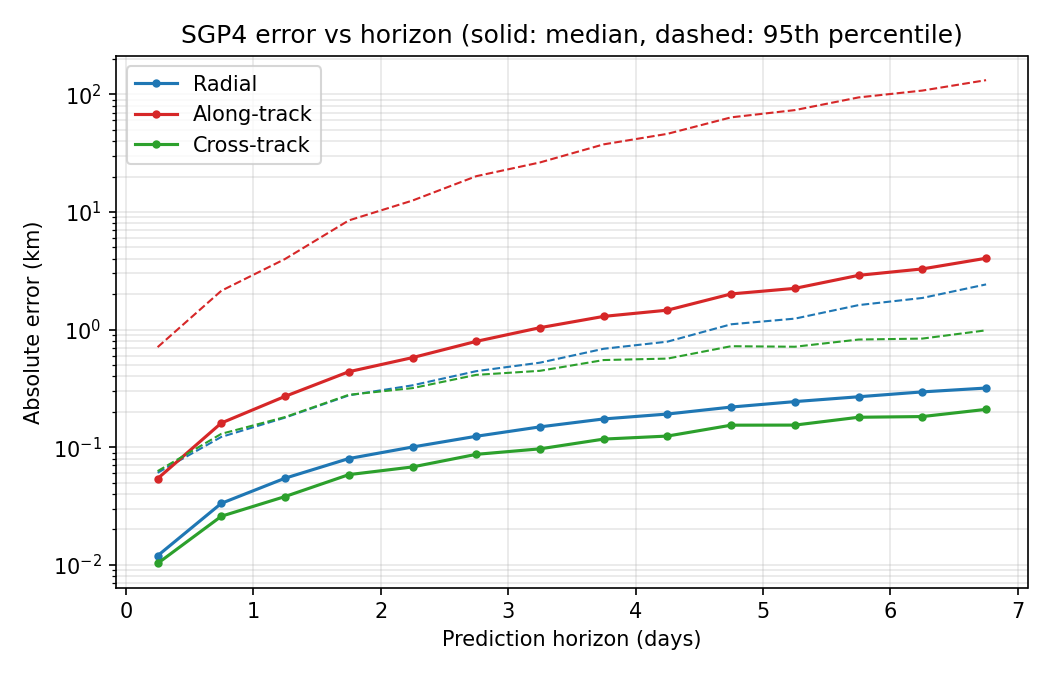
\includegraphics[width=0.6\textwidth]{checkpoint_error_growth.png}
\caption{SGP4 error against prediction horizon in RTN components, all 1.38 million pairs. Solid: median; dashed: 95th percentile.}
\label{fig:checkpoint}
\end{figure}



\subsection{Model inputs}

In order to represent a realistic application, all inputs use only information available at the epoch of element set $i$, meaning no future or data from the prediction window itself is incorporated into the model (Table~\ref{tab:inputs}). Space weather is taken from the last \emph{completed} day before the epoch, and the solar-flux average is the trailing 81-day mean.

\begin{table}[htbp]
\centering
\small
\captionsetup{width=0.8\linewidth}
\caption{Model inputs. All are numeric. ``Element set'' values are as published (OMM/TLE conventions).}
\label{tab:inputs}
\begin{tabular}{L{3.6cm}L{2.6cm}L{7.6cm}}
\toprule
Input & Units (domain) & Meaning \\
\midrule
Horizon & days (0--7] & Time from epoch $i$ to the prediction time \\
B* & 1/Earth radii & Fitted drag term of element set $i$ \\
Mean motion, its derivative & rev/day, rev/day$^2$ & Orbit size; rate of orbital decay \\
Eccentricity, inclination & --, degrees & Orbit shape and orientation \\
Perigee, apogee altitude & km (300--2000) & From mean motion and eccentricity (WGS72) \\
F10.7, 81-day average & solar flux units & Solar extreme UV heats the thermosphere \\
Ap, 3-day mean Ap & index & Geomagnetic activity; storms raise density \\
Previous error (R, T, N), gap & km, days & Error of an element set 1--3 days older, propagated to epoch $i$ \\
Previous drift rate & km/day$^2$ & Previous along-track error / gap$^2$ \\
B* change & 1/Earth radii & B* of $i$ minus B* of that older element set \\
\bottomrule
\end{tabular}
\end{table}

The ``previous'' features show how badly drag has recently been mis-estimated for this object. They are missing for 2.2\% of pairs, where no element set 1--3 days older exists.

\subsection{Outputs}

The model outputs a predicted SGP4 residual $(\Delta R, \Delta T, \Delta N)$ in km for a given element set and horizon. The corrected prediction is the SGP4 position minus this residual. The evaluation outputs are position-error statistics (median, 95th percentile, RMSE, in km) by altitude band and horizon, with bootstrap confidence intervals, saved as CSV files and figures in \texttt{reports/}. Function-level inputs and outputs are documented in the docstrings and the HTML documentation generated with pdoc (\texttt{docs/} in the repository).

\subsection{Invalid, missing and unsupported inputs}

Malformed element sets (non-numeric fields, unparseable epochs, eccentricity outside $[0,1)$, non-positive mean motion) are dropped and counted, as are pairs where SGP4 returns an error code (none occurred). For duplicate epochs the most recently created record is kept. Missing history features are passed to the trees as missing values, which gradient boosting handles natively, and set to zero for ridge. Pairs above the 99.9th percentile of error within their altitude band and 1-day horizon bin are identified, excluded from training and kept in all evaluation. Inputs that exist beyond the training domain are \emph{not} necessarily rejected automatically. Horizons beyond 7~days, perigees outside 300--2000~km, manoeuvring satellites and deep-space orbits lie outside the training domain, and the model will still return predictions for them. The application of this approach to inputs beyond the training domain is further discussed in Section~\ref{sec:7}.

%=====================================================================
\section{Computational Approach}\label{sec:3}
%=====================================================================

Both learned methods are extensions of regression methods taught in the MMA3001 unit, and the surrounding workflow applies the unit's material on evaluation, data selection as well as profiling (Table~\ref{tab:unit}).

\begin{table}[htbp]
\centering
\small
\captionsetup{width=0.8\linewidth}
\caption{Methods used and their relationship to unit content.}
\label{tab:unit}
\begin{tabular}{L{3.6cm}L{4.4cm}L{7.2cm}}
\toprule
Method in this project & Unit topic & Extension beyond the unit material \\
\midrule
Gradient boosting (selected) & 5.2 Decision Tree Regression & Ensemble of trees, each fitted to the previous trees' errors; absolute-error loss; horizon-scaled target \\
Ridge regression (alternative) & 5.1 Linear Regression; 3.2 Overfitting & L2 penalty on least squares; physics-derived regressors \\
Object- and time-based split & 5.6 Training Data Selection & Prevents leakage between correlated samples \\
Median, p95, RMSE, bootstrap & 5.5 Evaluating Regression & Confidence intervals resampling whole objects \\
Profiling, vectorisation & 2.1 Optimisation and Profiling & cProfile-guided speed-up, before/after timing \\
Unit tests & 1.5 Testing and Validation & 32 pytest tests (Appendix~\ref{app:tests}) \\
PINN, Runge--Kutta & 10.3 PINNs; 7.4 Runge--Kutta & Considered, not implemented (Section~\ref{sec:4}) \\
\bottomrule
\end{tabular}
\end{table}

\subsection{Gradient boosting}

The selected method is gradient-boosted regression trees, using scikit-learn's histogram-based implementation \cite{friedman2001,ke2017,pedregosa2011}. It extends the single decision-tree regressor of unit topic 5.2: one deep tree overfits noisy data (topic 3.2), whereas boosting adds many small trees in sequence, each correcting the errors of those before it. The model is a sum of $M$ small regression trees,
\begin{equation}
F_M(\mathbf{x}) = F_0 + \nu \sum_{m=1}^{M} h_m(\mathbf{x}),
\end{equation}
where each tree $h_m$ is fitted to the negative gradient of the loss at the current prediction and $\nu$ is the learning rate. With absolute-error loss, each tree is fitted to the sign of the current residual and its leaf values are set to medians, which makes the model robust to the heavy-tailed residuals in this data (the 99.9th percentile is 70--190 times the median in every band). Inputs are binned into 255 histogram bins, which is what makes training on 650,000 rows take under a minute.

One model is trained per RTN component. Previous work has corrected orbit predictions from public data with neural networks and support vector machines \cite{peng2018ann,peng2020}. Gradient boosting was chosen in this case because the data is tabular with mixed feature types, a setting where tree-based models are generally thought to outperform neural networks \cite{grinsztajn2022}. This is because the physics involves interactions (drag error depends jointly on altitude, space weather and elapsed time) that trees capture without them being specified explicitly. Further because missing values are handled directly, without the need for guessed substitute values, and because the model feature importance can be understood clearly.

\subsection{Physical constraint: zero correction at zero horizon}

An element set has no propagation error at its own epoch (i.e. at $t_{elapsed}=0$), so any correction must go to zero as the horizon $h \to 0$. Rather than leaving the model to learn this, it is built into the model itself. The trees learn the residual per day of horizon, $g(\mathbf{x}) \approx \Delta/\tau$, with $\tau = \max(h, 1\,\text{h})$ to avoid division by near-zero horizons, and each sample is weighted by $\tau$. Because
\begin{equation}
\sum_k \tau_k \left| \frac{\Delta_k}{\tau_k} - g(\mathbf{x}_k) \right| = \sum_k \left| \Delta_k - \tau_k\, g(\mathbf{x}_k) \right|,
\end{equation}
this still minimises absolute error in km, while the prediction $\tau g(\mathbf{x})$ shrinks to near zero at short horizons.

\subsection{Physics terms}

A constant error $\Delta\dot{n}$ in the rate of change of mean motion gives an along-track error
\begin{equation}
\Delta s(t) \approx \tfrac{1}{2}\, a\, \Delta\dot{n}\, t^2,
\end{equation}
where $a$ is the semi-major axis \cite{vallado2013}. Interaction terms built on this form (horizon$^2$, B*$\times$horizon$^2$, previous drift rate $\times$ horizon and $\times$ horizon$^2$, previous errors $\times$ horizon) are added to the inputs of both learned models. This is because the growth law is already known and therefore doesn't need to be relearned by the model.

\subsection{Training, validation and test split}

Pairs from the same object are strongly correlated, so a random split, as used for independent samples in unit topic 5.6, would leak information between training and test data sets. The split is therefore by object and by time. Objects are assigned 70/15/15\% to training, validation and test within each altitude band (168/39/39 objects). Training pairs end before 30~December 2025; validation uses the validation objects from then until 31~March 2026; the test set is the test objects from 31~March 2026 onwards. This gives 653,011 training, 33,605 validation and 30,738 test pairs. Every test result is on objects the model has never seen, in a period it has never seen.

\subsection{Settings and model development}

Hyperparameters were chosen by a random search of eight configurations on a 150,000-row training sample, scored by along-track validation mean absolute error (MAE). The model was first trained with up to 300 trees, then retrained using whichever number of trees had given the lowest validation error. The selected settings were learning rate 0.05, maximum 127 leaves per tree, minimum 50 samples per leaf and no L2 penalty, giving 132, 172 and 230 trees for the R, T and N components.

The model went through three iterations, each driven by a diagnosed failure (Table~\ref{tab:runs}):
\begin{enumerate}
\item \textbf{Run 1:} validation objects shared the training period. Tuning rewarded models that memorised conditions of that period, for example through the slowly varying 81-day solar flux, which effectively encodes the date. On the test period the correction made median error 22\% worse.
\item \textbf{Run 2:} validation moved to its own period between training and test data sets. The model now beat no correction on validation, and test RMSE fell 12\%, but short-horizon errors were still large due to the lack of a zero-horizon constraint.
\item \textbf{Run 3 (final):} the zero-horizon constraint above was added to both learned models.
\end{enumerate}

\begin{table}[htbp]
\centering
\small
\captionsetup{width=0.8\linewidth}
\caption{Model iterations. Validation: along-track MAE; test: 3-D position error over all test pairs (km).}
\label{tab:runs}
\begin{tabular}{lcccc}
\toprule
 & Val.\ MAE & Test median & Test p95 & Test RMSE \\
\midrule
SGP4 (no correction) & 17.82 & 0.582 & 30.29 & 22.07 \\
Run 1: shared val.\ period & 11.57 & 0.712 & 34.48 & 20.88 \\
Run 2: separate val.\ period & 16.71 & 0.638 & 28.83 & 19.48 \\
Run 3: + zero-horizon constr. & 16.55 & 0.665 & 29.49 & 19.31 \\
\bottomrule
\multicolumn{5}{l}{}
\end{tabular}
\end{table}

\textbackslash{}textbf\{Assumptions.\} SGP4's error is assumed to be partly predictable from information available at epoch, and the relationship learned from 168 objects and one period is assumed to transfer to similar objects and later periods.

%=====================================================================
\section{Alternative Solutions}\label{sec:4}
%=====================================================================

One alternative solution was implemented and one more was considered but ultimately rejected.

\textbf{Baseline: uncorrected SGP4.} This is the real-world standard and therefore the reference that any corrections made by this work must perform better than.

\textbf{Alternative: ridge regression on physics terms.} This extends the linear least-squares regression of unit topic 5.1 by adding an L2 penalty on the coefficients, a standard control for the overfitting covered in topic 3.2: $\min_\beta \|\mathbf{y} - X\beta\|^2 + \alpha\|\beta\|^2$, on the eight horizon-proportional physics terms, with no intercept and the regularisation strength $\alpha$ chosen on validation from $10^0$ to $10^4$. It tests whether the known drag-growth law, with coefficients fitted from data, is enough on its own.

\textbf{Considered and not implemented.} A numerical propagator integrating gravity, J2 and drag with a Runge--Kutta method (unit topic 7.4), started from SGP4's position and velocity at epoch, would replace SGP4 rather than correct it. It was not implemented within the project timeline, and it would face the same dominant error source, since the drag coefficient must still be estimated from the element set; it remains a worthwhile numerical baseline for future work.

%=====================================================================
\section{Validation}\label{sec:5}
%=====================================================================

\subsection{What was validated and how}

\textbf{Verification of the implementation.} All 32 automated tests pass (pytest; summarised in Appendix~\ref{app:tests}, with full results in \texttt{reports/test\_report.html}). They check that the RTN frame conversion is correct, that element sets are loaded exactly as the standard TLE reader loads them (to within 1~mm over 7~days), that every residual matches a separate SGP4 calculation, that no future information is given to the space-weather inputs or the data split, that both corrections are zero at zero horizon, that the models can learn a known pattern in made-up data, and that the faster code gives the same results as the original. Figure~\ref{fig:checkpoint} also confirms that the errors behave as the underlying physics predicts.

\textbf{Validation of the model.} The model was tested on data never seen during training or tuning with 39 objects being used over a final three-month period. Because most errors are small but a few are very large, three measures of 3-D position error were recorded. These were the \emph{median} (a typical error), the \emph{95th percentile} (the bad cases) and the \emph{RMSE}, which is driven mostly by the largest errors, the ones that matter most for collision avoidance for example. Confidence intervals come from a bootstrap that repeatedly resamples whole objects (500 times) \cite{efron1993}, because pairs from the same object are not independent.

\subsection{Results}

\begin{table}[htbp]
\centering
\small
\caption{Reduction in test position error relative to SGP4 (positive is better), with 95\% bootstrap confidence intervals over objects.}
\label{tab:bootstrap}
\begin{tabular}{lccc}
\toprule
Method & Median & 95th percentile & RMSE \\
\midrule
Gradient boosting (GB) & $-14.3\%$ ($-36.0$ to $3.1$) & $2.6\%$ ($-3.6$ to $6.2$) & $\mathbf{12.5\%}$ \textbf{(4.4 to 17.1)} \\
Ridge & $-128.9\%$ ($-211.4$ to $-58.7$) & $0.6\%$ ($-2.2$ to $2.2$) & $-0.4\%$ ($-1.9$ to $-0.1$) \\
\bottomrule
\end{tabular}
\end{table}

\begin{table}[htbp]
\centering
\small
\caption{Test position error by perigee band (km).}
\label{tab:bands}
\begin{tabular}{lccccccccc}
\toprule
 & \multicolumn{3}{c}{Median} & \multicolumn{3}{c}{95th percentile} & \multicolumn{3}{c}{RMSE} \\
\cmidrule(lr){2-4}\cmidrule(lr){5-7}\cmidrule(lr){8-10}
Band (km) & SGP4 & Ridge & GB & SGP4 & Ridge & GB & SGP4 & Ridge & GB \\
\midrule
300--500   & 4.63 & 4.65 & 4.81 & 68.5 & 68.3 & \textbf{63.5} & 38.6 & 38.8 & \textbf{33.6} \\
500--700   & 1.73 & 1.93 & 1.97 & 38.8 & 38.0 & \textbf{34.0} & 21.2 & 21.2 & \textbf{19.0} \\
700--900   & 0.34 & 0.79 & 0.45 & 2.25 & 4.51 & 2.91 & 1.19 & 2.09 & 1.50 \\
900--1200  & 0.35 & 0.86 & \textbf{0.31} & 2.09 & 4.22 & 2.18 & 1.07 & 1.98 & 1.09 \\
1200--2000 & 0.30 & 0.97 & \textbf{0.26} & 3.17 & 5.58 & 3.65 & 5.34 & 5.46 & 5.60 \\
\bottomrule
\end{tabular}
\end{table}

\begin{figure}[htbp]
\centering
\captionsetup{width=0.8\linewidth}
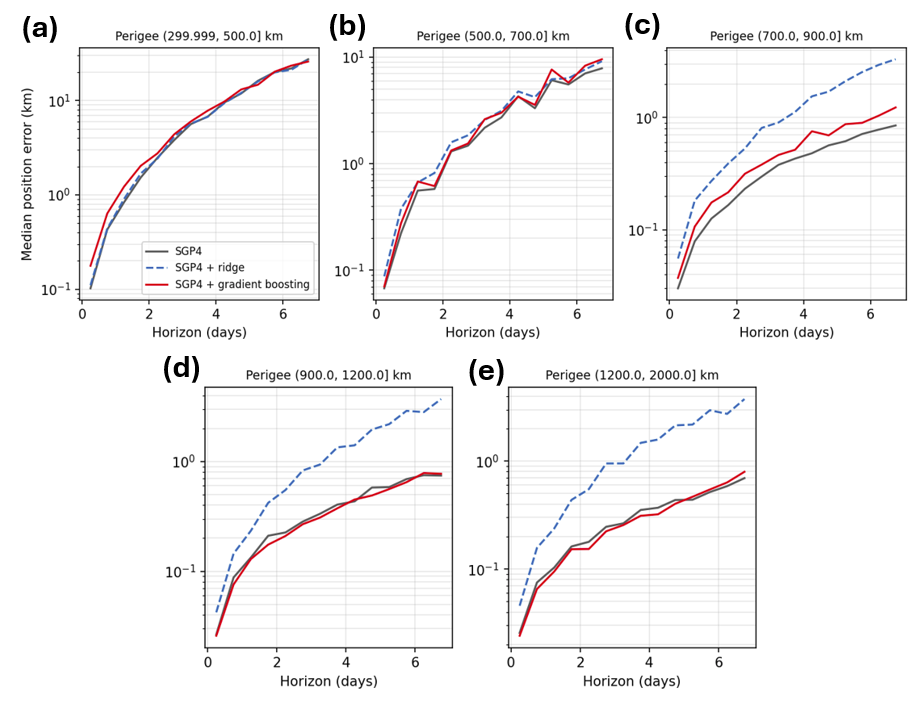
\includegraphics[width=0.7\textwidth]{error_growth_by_band.png}
\caption{Median test position error against prediction horizon for SGP4 alone, SGP4 with the ridge correction and SGP4 with the gradient-boosting correction, by perigee band: (a)~300--500~km, (b)~500--700~km, (c)~700--900~km, (d)~900--1200~km and (e)~1200--2000~km. Note the different vertical scales.}
\label{fig:growth}
\end{figure}

The main result observed was that gradient boosting was seen to reduce RMSE by 12.5\% with a confidence interval entirely above zero (Table~\ref{tab:bootstrap}). These gains are seen to be concentrated in the two lowest bands, where RMSE fell from 38.6 to 33.6~km and from 21.2 to 19.0~km, and the 95th percentile fell by 7\% and 12\% (Table~\ref{tab:bands}). Overall, the 95th-percentile and median changes are not significant, so the improvement comes from the largest errors, beyond the 95th percentile. Typical errors were not seen to have improved. In the lowest band, the median at horizons under one day rose from 0.24 to 0.40~km, and the 700--900~km band was worse on each measure. Above 900~km the median improved only slightly (Figure~\ref{fig:growth}).

Ridge regression unfortunately made the median worse in every band and gave no RMSE improvement. With one set of coefficients across all altitudes, its fit is dominated by the large low-altitude errors and then applied to orbits where errors are 40 times smaller, adding up to 2~km at 5--7~days above 700~km. Its validation-selected regularisation was the strongest available ($\alpha = 10^4$) for the radial and along-track components, meaning the data favoured shrinking it towards no correction at all.

\subsection{Interpretation}

Permutation importance \cite{breiman2001} on the test set (Figure~\ref{fig:importance}) shows the model relies on evidence that the drag estimate is wrong. The top five inputs being the change in B* since the previous element set, the recent along-track drift rate, the horizon, the geomagnetic Ap index, and the mean motion derivative (orbital decay rate). This matches the physics. A sudden change in the fitted B* means the drag estimate is unsettled, recent drift shows the current estimate is inaccurate and geomagnetic storms heat the thermosphere, therefore raising density beyond what is assumed by B* \cite{picone2002}.

The solar flux (F10.7) features have slightly negative importance and shuffling them makes predictions marginally better. Solar flux varies over months, so the model likely used it to identify the time period rather than to learn about drag. This was found on the test set, so the features were not changed afterwards.

This also explains where the correction helps. Below 700~km, drag dominates and its mis-estimation leaves detectable traces in the recent history, so the largest errors are partly predictable. Above 900~km drag is weak, errors flatten to a floor of a few hundred metres set by noise in the element-set fits themselves, and there is little systematic signal to learn.

\begin{figure}[htbp]
\centering
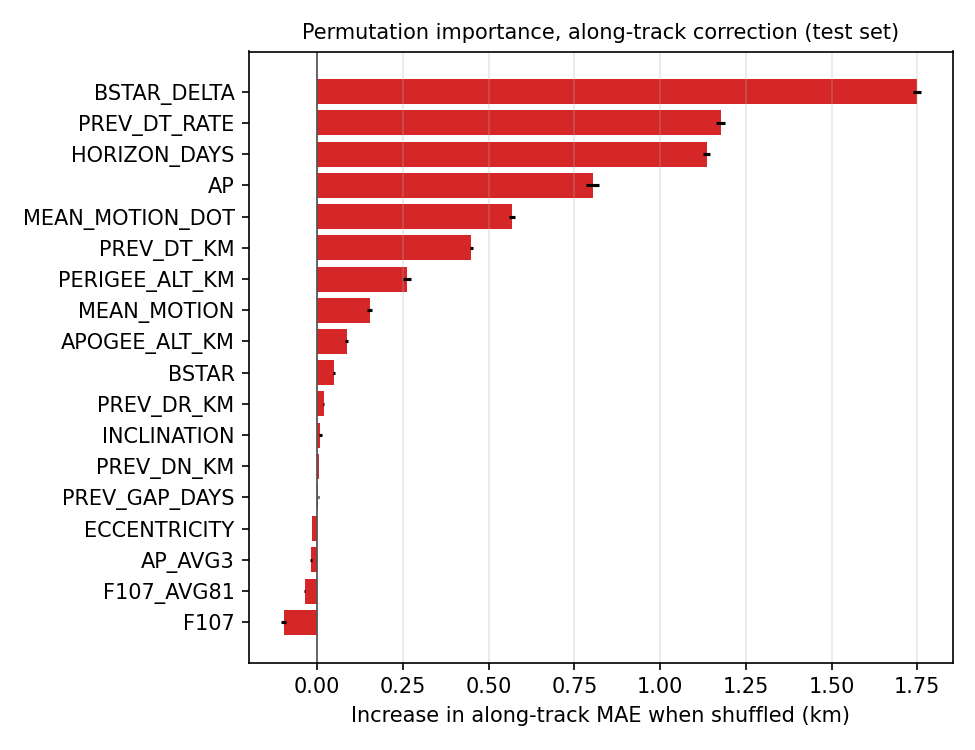
\includegraphics[width=0.55\textwidth]{feature_importance.png}
\captionsetup{width=0.8\linewidth}
\caption{Permutation importance for the along-track correction: increase in test MAE when each input is shuffled (reference MAE 5.85~km). Inputs indicating drag mis-estimation rank highest; the F10.7 features rank below zero.}
\label{fig:importance}
\end{figure}

\subsection{What the validation cannot establish}

\begin{itemize}
\item \textbf{True position accuracy.} The reference is another element set, so the results show the correction makes predictions more consistent with the \emph{next} TLE, not closer to the satellite's true position. Precise ephemerides (for example, laser-ranged satellites) would be needed for that.
\item \textbf{Generality across time.} The test period is a single three-month window (April--June 2026) at one phase of the solar cycle. Performance in quieter conditions, or during storms more extreme than the training data (maximum Ap 144), is unknown.
\item \textbf{Generality across objects.} With 39 test objects (7--8 per band), per-band results are uncertain, and objects outside the selected population are untested.
\end{itemize}

%=====================================================================
\section{Optimisation and Performance}\label{sec:6}
%=====================================================================

\subsection{Runtime, memory and work per prediction}

Runtimes were measured with \texttt{time.perf\_counter} as the best of several repeats, on a laptop with an Intel(R) Core(TM) Ultra 5 225H processor running Python 3.14 on Windows (Table~\ref{tab:perf}).

\begin{table}[htbp]
\centering
\small
\caption{Runtime and size. Batched times are per prediction for all three RTN components.}
\label{tab:perf}
\begin{tabular}{lcccc}
\toprule
 & Batched ($\mu$s) & Single call & Size & Work per prediction \\
\midrule
SGP4 propagation & 0.38 & 0.38 $\mu$s & -- & -- \\
Ridge & 0.51 & 5.8 ms & 5 KB & $\approx$96 FLOPs \\
Gradient boosting & 4.77 & 11.0 ms & 7.6 MB & $\approx$4,400 comparisons + 534 adds \\
\bottomrule
\end{tabular}
\end{table}

Gradient boosting costs 12.5 times one SGP4 call, but still processes about 200,000 predictions per second on one core. A single prediction takes 11\~ms of library overhead, so a theoretical deployed system should process predictions in batches. Its 534 trees hold 135,102 nodes (about 57 bytes each), and each node visit loads a record to perform one comparison, roughly one operation per 50~bytes of memory. With 7.6~MB of trees, larger than a typical L2 cache, inference is bound by memory latency and branching rather than arithmetic.

\subsection{Profiling-driven optimisation}

Following the profiling approach of unit topic 2.1, \texttt{cProfile} showed the history features dominated the workflow. Each residual was rotated into RTN with a separate call, 1,541 rotations taking 0.193~s of 0.374~s for one object. The improved version rotates all states in one array operation, with a test confirming identical results. History features ran 5.3 times faster (0.44~s to 0.08~s on 6,987 element sets), the per-object pipeline 2.4 times faster (0.374~s to 0.156~s), and function calls fell from 438,203 to 99,651, leaving no single dominant cost.

\subsection{Sensitivity}

All eight hyperparameter configurations beat no correction on validation (MAE 16.66--17.03~km against 17.82~km). Their 2.2\% spread is smaller than the gain over SGP4, so results are not sensitive to these settings. They are far more sensitive to validation design. I.e. separating validation in time from training (run 1 to run 2, Table~\ref{tab:runs}) reversed the conclusion. Altitude and horizon sensitivity are shown in Table~\ref{tab:bands} and Figure~\ref{fig:growth}, and excluding flagged outliers changes only the top band without changing which method is better. Sensitivity to the amount of training data, and training on low bands while testing on high ones, was not performed but is identified as a future avenue of sensitivity analysis.

\subsection{Selected design}

Gradient boosting is selected because it is the only method that reduced error on any measure, at an acceptable cost of a few microseconds per prediction. Ridge however, despite being faster and smaller, cannot represent the altitude dependence of the error. The recommended deployment is batch correction below 700~km and beyond one day's horizon, a gating rule that should first be confirmed on validation data, since it was identified from test results.

%=====================================================================
\section{Limitations and Lessons Learned}\label{sec:7}
%=====================================================================

\textbf{Limitations.} Beyond the improvements in large errors identified in Section~\ref{sec:5}, the correction is not necessarily seen to improve overall typical error, and adds a few hundred metres at short horizons in LEO. The weakest point is an object that has just manoeuvred or broken apart, because its recent history no longer matches its current orbit. A real system might detect sudden changes in B* and skip the correction for those objects. The model also cannot know what space weather will occur during the prediction, which presents as a limitation to how much the correction can ever improve.

\textbf{Lessons learned.}
\begin{enumerate}
\item \textbf{Validation design matters more than model tuning.} A validation set that shared the training period produced confident but wrong model choices; separating it in time changed the conclusion from ``the correction makes things worse'' to ``the correction helps the largest errors''.
\item \textbf{Physical constraints are cheap and effective.} Building in the requirement that the correction vanish at zero horizon fixed most of the bad performance for short-horizons in ridge without any tuning.
\item \textbf{One summary statistic can mislead.} The same model is 12.5\% better by RMSE and 14\% worse by median. When most errors are small but a few are very large, the right measure depends on whether the application cares more about typical errors or the worst case scenario errors.
\end{enumerate}

\textbf{Proposed improvements,} in order of expected value: validate against precise ephemerides for a subset of objects. Fit separate models or add gating by altitude regime, chosen on validation data. Add forecast space weather as an input. Implement a Runge--Kutta propagator (topic 7.4) as a numerical baseline, with a step-size convergence study. Run the training-size and altitude-generalisation studies. Add explicit input-domain checks.

%=====================================================================
\section{AI Use and Reflection}\label{sec:ai}
%=====================================================================

\textbf{Tools, use and level of contribution.} The project concept, scope and method (a machine-learning correction of SGP4 residuals, validated across prediction horizons and orbit regimes) were set out in my initial proposal before any AI use. I then used Claude (Anthropic, via the Claude app, October 2026) as a tool under my direction to critique that proposal, draft the source modules and tests stage by stage as I requested them, to troubleshoot PowerShell, Git and GitHub problems, and to draft this report from my results. It drafted the initial code and a first draft of the report structure. I ran every stage on my own data, checked each result before moving to the next, and decided whether to adopt each proposed change, rejecting some (see final paragraph).

\textbf{How AI output was checked.} I ran every stage on my own machine and data. Every module has unit tests, run before results were used; the checkpoint plot (Figure~\ref{fig:checkpoint}) had to show physically sensible error growth before modelling; and results were compared with an uncorrected baseline.

\textbf{Errors and unhelpful suggestions.} The most consequential was the AI's original split, which put validation in the same period as training; run~1 showed the correction making test error worse, and the cause was traced to this design decision made by the AI. Its first models also lacked the zero-horizon constraint, and its ridge model had an intercept, inflating short-horizon errors. It also gave numerous Linux shell commands that failed in PowerShell.

\textbf{Effect on my understanding, and decisions that remained mine.} AI changed where I spent my effort. Less was spent on writing code and more was spent on checking it as well as interpreting results. Because I verified its output through tests and physical checks rather than line by line, the results became my main way of understanding the problem. Run~1 taught me that AI-designed validation can look sound and yet still be problematic, and the error-growth plot (Figure~\ref{fig:checkpoint}) taught me why along-track error dominates. The key decisions however were mine. I.e. the topic and LEO scope, accepting TLE as a ground truth with its limitation stated, and when to stop iterating on aspects of the project. The cost of using AI in this way was a shallower grasp of some implementation details than if I had written the code entirely myself.

\clearpage

\begin{appendices}

\section{Bibliography}\label{sec:bib}

\printbibliography[heading=none]

\clearpage

\section{Dataset by Perigee Band}\label{app:data}

\begin{table}[htbp]
\centering
\caption{Dataset by perigee band. Along-track error is SGP4's median absolute error for 5--7 day horizons across all pairs.}
\label{tab:data}
\begin{tabular}{lrrr}
\toprule
Perigee band (km) & Objects & Element sets & Along-track error, 5--7 d (km) \\
\midrule
300--500   & 50 & 90,290 & 26.1 \\
500--700   & 50 & 64,912 & 7.3 \\
700--900   & 46 & 63,530 & 2.0 \\
900--1200  & 50 & 71,955 & 0.7 \\
1200--2000 & 50 & 60,323 & 0.6 \\
\bottomrule
\end{tabular}
\end{table}

\section{Hyperparameter Search}\label{app:search}

\begin{table}[htbp]
\centering
\caption{Random search, run 3 (along-track validation MAE; uncorrected 17.82~km).}
\begin{tabular}{ccccc}
\toprule
Learning rate & Max leaves & Min leaf size & L2 & Validation MAE (km) \\
\midrule
0.05 & 127 & 50  & 0  & \textbf{16.662} \\
0.10 & 31  & 50  & 0  & 16.696 \\
0.05 & 127 & 200 & 0  & 16.711 \\
0.03 & 127 & 50  & 10 & 16.747 \\
0.10 & 63  & 200 & 10 & 16.805 \\
0.10 & 63  & 50  & 10 & 16.809 \\
0.20 & 63  & 50  & 0  & 16.912 \\
0.05 & 15  & 20  & 0  & 17.029 \\
\bottomrule
\end{tabular}
\end{table}

\section{Automated Tests}\label{app:tests}

\begin{table}[htbp]
\centering
\small
\begin{tabular}{L{3.2cm}L{11.5cm}}
\toprule
Module & What the tests confirm \\
\midrule
\texttt{frames.py} & RTN basis is orthonormal and right-handed; a pure shift along each axis lands only in that component; rotation preserves length; degenerate states raise errors. \\
\texttt{pairs.py} & Element-set loader matches the library's TLE parser to 1~mm over 7~days; malformed and duplicate records are dropped; an object placed ahead in its orbit shows positive along-track error equal to the arc length; every residual matches a direct SGP4 computation; pairing respects the horizon limit and is reproducible. \\
\texttt{features.py} & Perigee/apogee altitude for the ISS is correct; space weather uses only completed days; history features select the right earlier element set; vectorised and original code agree; outlier flags are relative to band and horizon. \\
\texttt{models.py}, \texttt{evaluate.py} & Train, validation and test sets share no objects and are ordered in time; both models recover a known relationship in synthetic data; both corrections vanish at zero horizon; bootstrap intervals contain their estimates. \\
\texttt{performance.py} & Timing is positive; tree statistics are consistent; permutation importance identifies the informative feature in synthetic data. \\
\bottomrule
\end{tabular}
\end{table}

\end{appendices}

\end{document}